\section{Chimera Operate protocol}
\label{app:chimeraOperate}%a020

Protocol designed to perform operations with atomic structures in \scipion by using \chimera. A volume or set of volumes can also be included. Structures or maps generated by using this protocol can be saved in \scipion after executing specific \chimera commands. \chimera \ttt{rigid fit} protocol constitutes a particular case of this protocol to perform rigid fitting in \scipion by using \chimera (Appendix \ref{app:chimeraRigidFit}).

 \begin{itemize}
  \item Requirements to run this protocol and visualize results:
    \begin{itemize}
        \item \scipion plugin: \ttt{scipion-em-chimera}
    \end{itemize}
  \item \scipion menu:\\
   \ttt{Model building -> Tools-Calculators} (\ffigure{fig:app_protocol_chimera_2} (A))
  
  \item Protocol form parameters (\ffigure{fig:app_protocol_chimera_2} (B)):
  
    \begin{figure}[H]
     \centering 
     \captionsetup{width=.7\linewidth} 
     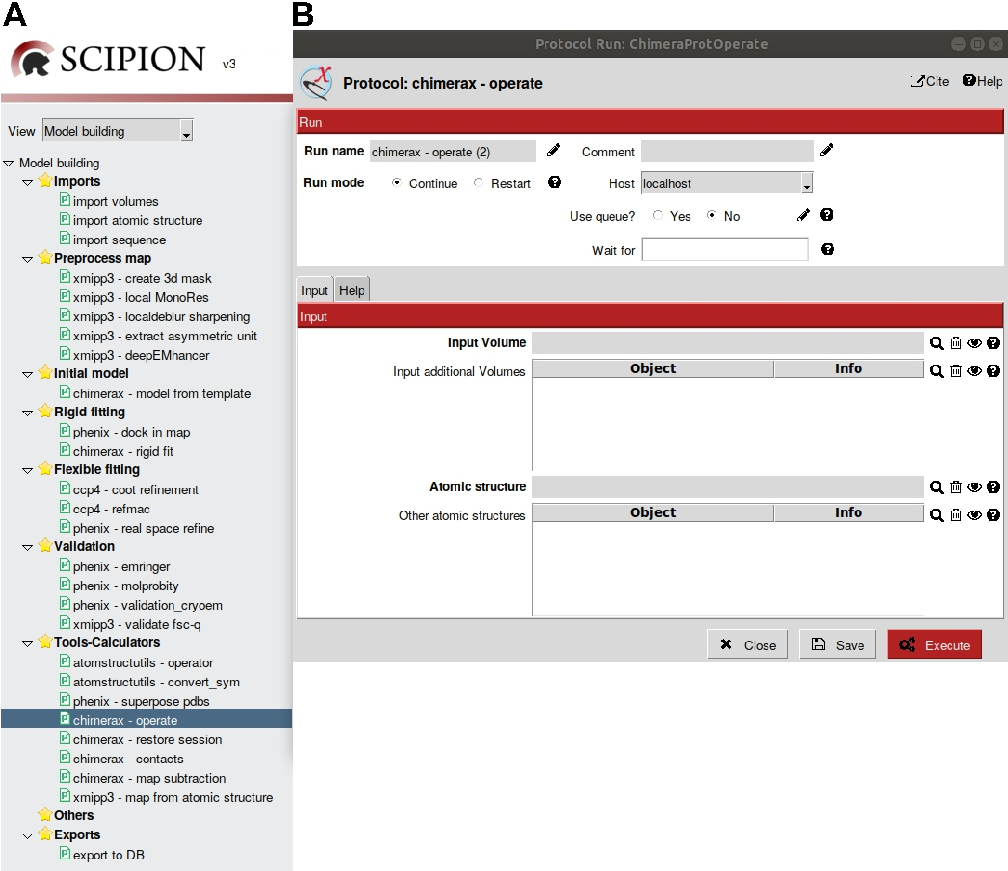
\includegraphics[width=0.90\textwidth]{Images_appendix/Fig117.pdf}
     \caption{Protocol \scommand{chimera operate}. A: Protocol location in \scipion menu. B: Protocol form.}
     \label{fig:app_protocol_chimera_2}
    \end{figure}
    
    \begin{itemize}
     \item \ttt{Input} section

    \begin{itemize}
     \item \ttt{Input Volume}: Optional parameter to be completed with the electron density map previously downloaded or generated in \scipion.
     \item \ttt{Atomic structure}: Atomic structure previously downloaded or generated in \scipion.
     \item \ttt{Other atomic structures}: Additional atomic structures.
    \end{itemize}
    \item \ttt{Help} section
    
    This section contains \chimera commands required to save $models$ according to their reference volumes, which can also be saved if required. Remark that using \ttt{scipionwrite} command, \chimera session will be saved by default, without prejudice that it may be saved with \ttt{scipionss} command. \chimera sessions can be restored by using \scommand{chimera restore session} protocol.
    
    \end{itemize}

  \item Protocol execution:\\
  
  Adding specific protocol label is recommended in \ttt{Run name} section, at the form top. To add the label, open the protocol form, press the pencil symbol at the right side of \ttt{Run name} box, complete the label in the new opened window, press OK and, finally, close the protocol. This label will be shown in the output summary content (see below). If you want to run again this protocol, do not forget to set to \ttt{Restart} the \ttt{Run mode}.\\
  Press the \ttt{Execute} red button at the form bottom.\\
  
  \chimera graphics window will be opened after executing the protocol. Electron density map, if loaded, and the atomic structure(s) are shown. Steps to follow depend on the specific operation to carry out. Usually, new volumes or structures are generated, and they have to be saved in \scipion.
  \begin{itemize}
   
   \item To save an atomic structure generated with this \chimera protocol:
   Write in \chimera command line:\\
   \ttt{scipionwrite model \#n}\\
   If you want to save the model regarding any electron density map, write in \chimera command line:\\
   \ttt{scipionwrite model \#n refmodel \#n saverefmodel 0/1}.\\Replace \ttt{\#n} by model numbers shown in \chimera \ttt{Model Panel}. After \ttt{saverefmodel}, select \ttt{1} if you want to save the reference map or \ttt{0} otherwise, to avoid duplicate data unnecessarily.
   \item To save a volume generated with this \chimera protocol:
   New volume data sets have to be saved first in a separate volume file. Otherwise, those volumes will not be saved in the \chimera session since session files only record file paths to volumes. Assuming that the name chosen for the new volume generated is \ttt{volume\_name.mrc}, and \ttt{abspath} the absolute path in which you want to save the volume, write in \chimera command line:\\
   \ttt{volume \#n save abspath/volume\_name.mrc}\\
   \ttt{scipionwrite model \#n refmodel \#n saverefmodel 1}.\\Replace \ttt{\#n} by model numbers shown in \chimera \ttt{Model Panel}. Remark that you have to save an atomic structure if you want to save a volume in \scipion.
   \item Close \chimera graphics window.

 \end{itemize}
  \item Visualization of protocol results:
  
    After executing the protocol, press \ttt{Analyze Results} and \chimera graphics window will be opened by default. Atomic structures and volumes are referred to the origin of coordinates in \chimera. To show the relative position of atomic structure and electron density volume, the three coordinate axes are represented; X axis (red), Y axis (yellow), and Z axis (blue) (\ffigure{fig:app_protocol_volume_3}). Coordinate axes, volume, and atomic structure are model numbers \ttt{\#0}, \ttt{\#1}, and \ttt{\#2}, respectively, in \chimera \ttt{Model Panel}. If no volumes have been included, coordinate axes and each atomic structure are model numbers \ttt{\#0} and \ttt{\#1}, respectively.
    
    \begin{figure}[H]
   \centering 
    \captionsetup{width=.7\linewidth} 
    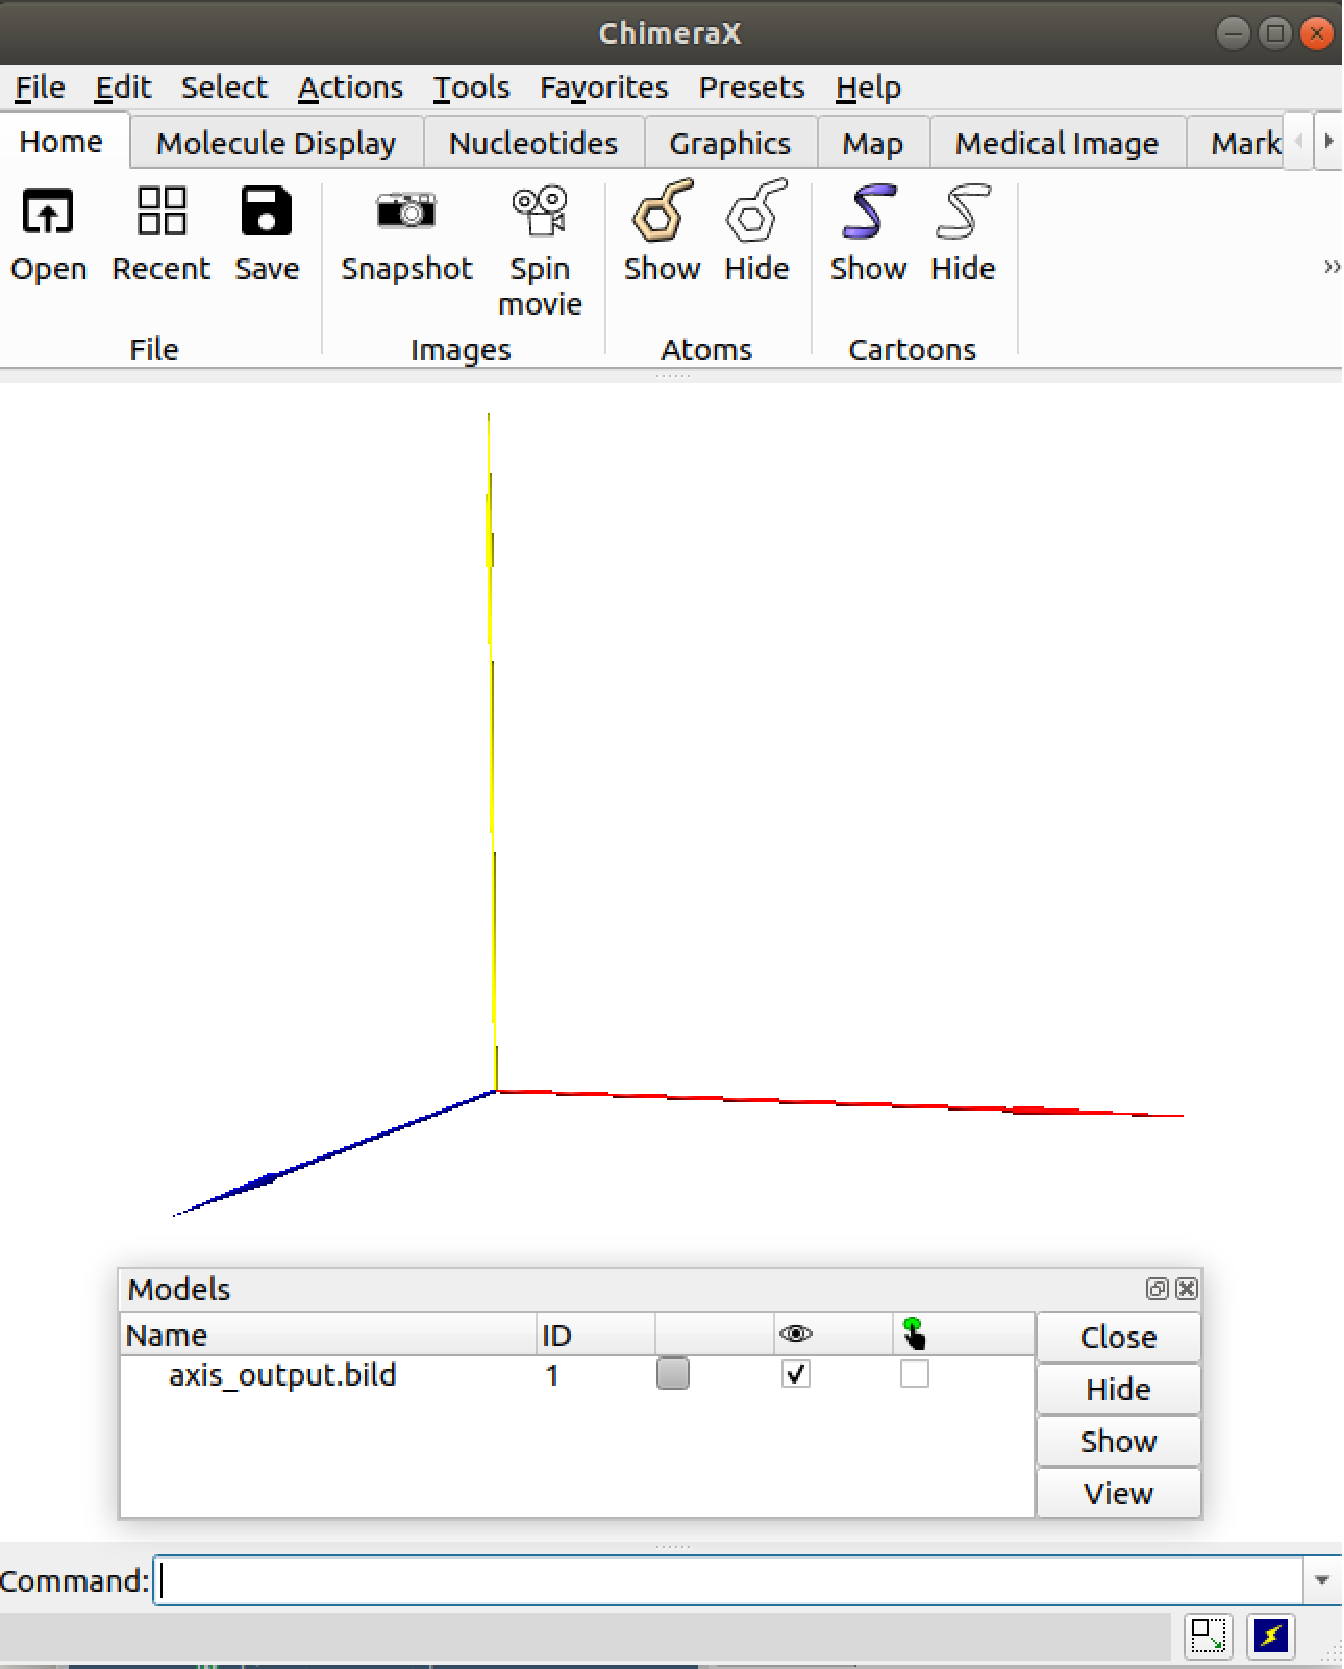
\includegraphics[width=0.75\textwidth]{Images_appendix/Fig102.pdf}
    \caption{Default $Chimera$ graphics window with coordinate axes.}
    \label{fig:app_protocol_volume_3}
    \end{figure}
   
  \item Summary content:\\
  
   \begin{itemize}
    \item If an atomic structure is generated:

    \begin{itemize}
     \item Protocol output (below \scipion framework):\\
      \ttt{chimera - chimera operate -> ouputPdb\_01}; \ttt{AtomStruct (pseudoatoms=True/ False, volume=True/ False)}.\\Pseudoatoms is set to \ttt{True} when the structure is made of pseudoatoms instead of atoms. Volume is set to \ttt{True} when an electron density map is associated to the atomic structure.
     \item \ttt{SUMMARY} box:\\Produced files:\\chimeraOut0001.pdb\\we have some result
    \end{itemize}
    \item If a volume is generated:
    
    \begin{itemize}
     \item Protocol output (below \scipion framework):\\
      \ttt{chimera - chimera operate -> ouput3Dmap}; \ttt{Volume (x, y, and z dimensions, sampling rate)}.\\
      \ttt{chimera - chimera operate -> ouputPdb\_01}; \ttt{AtomStruct (pseudoatoms=True/ False, volume=True/ False)}.\\Pseudoatoms is set to \ttt{True} when the structure is made of pseudoatoms instead of atoms. Volume is set to \ttt{True} when an electron density map is associated to the atomic structure.
     \item \ttt{SUMMARY} box:\\Produced files:\\chimeraOut0001.pdb\\chimeraOut0001.mrc\\we have some result
    \end{itemize}
    
   \end{itemize}
  
 \end{itemize}

